\chapter{The~\texttt{porthos2}:~implementation}
\label{ch:impl}

% function invocations/calls: inlining with binding
% contexts: for now, no ctxs
% comparing to cprover (https://www.cprover.org/cbmc/doc/manual.pdf, page 45, absatz about 'goto') where "the loop is unwound a given number of times" , we SHOULD have 2 modes of unrolling: 1) number of times, and 2) number of high-level instructions executed
% TODO(code): (https://www.cprover.org/cbmc/doc/manual.pdf, page 45) "The break and continue statements are replaced by equivalent goto statements as described in the ANSI-C standard."

% TODO: arrays: cprover manual page 48

Current Chapter describes the architecture of the \porthos[2] framework.

The programming language choice for \porthos[2] was made in favour of java in order to be able to reuse some parts of its predecessor \porthos written in java.
However this language does not show best results in performance benchmarks (comparing to C++, for example)~\cite{TODO}, the performance cornerstone of \porthos[2] (as well as any other SMT-based code analyser) is the phase of solving the SMT-formula, which is left to the third-party SMT-solver called from \porthos[2] via java API.
However, considering the perspective of using \porthos[2] as a static analyser for real-world programs, the memory optimisation problem must also be taken into account during both encoding and solving stages.


\section{Requirements}
\label{ch:impl:req}

The main reason for starting the work on re-implementing the \porthos tool was the need for extension the input language and optimisation of the tool so that it is able to process real C programs in perspective.
In the existing \porthos architecture, the high-level recursive instructions (statements of C) are processed together with low-level non-recursive events abstractions (see classes of package `\texttt{dartagnan.program}' of \porthos) as single AST structure.
This AST was implemented as a mutable data structure, which is being modified during the stage of SMT-encoding.
We consider this architecture as hardly manageable (since it is hard to guarantee preserving of the invariants during the program execution) and poorly extensible (since adding support for a new high-level control-flow instruction requires changing multiple components of the program, from parser to encoder).
%Moreover, we encounter serious problems when we need to add support for control-flow jumps (as \texttt{continue}, \texttt{break}, \texttt{goto} in C).

Therefore, while designing the architecture of \porthos[2], we decided to clearly separate the high-level intermediate code representation (implemented as a recursive AST structure) from low-level event-based representation (implemented as an event-flow graph).
Such a modular architecture allows to use multiple input language parsers and convert parsed syntax trees to our AST, thus having support for multiple languages (for instance, the original input language of \porthos tool, two variants of syntax of a litmus test used by \tool{herd}, an assembly language for any supported architecture).

The following list enumerates the target \textit{requirements} for the new tool:

\begin{enumerate}[nolistsep]
    \item \textit{stability and transparency}
        \begin{itemize}
            \item following the principles of simplicity and readability;
            \item usage of software design patterns if necessary;
            \item usage of immutable data structures for all data transfer objects~(DTO);
            \item high code coverage by unit and functional tests;
        \end{itemize}
    \item \textit{efficiency}
        \begin{itemize}[leftmargin=1em]
            \item keeping the trade-off between execution time and memory usage;
        \end{itemize}
    \item \textit{extensibility}
        \begin{itemize}[leftmargin=1em]
            \item clear modular architecture
        \end{itemize}
\end{enumerate}


\section{Program Components}
\label{ch:impl:comp}

The general architecture of \porthos[2] is presented in Figure~\ref{fig:program-components}.
The program receives as input the program to be analysed (see Section~\ref{ch:impl:input}) and one (the reachability analysis mode) or two (the portability analysis mode) memory models (see Section~\ref{ch:impl:input-parser}).
Then, the parsed program input (called Y-tree%
\footnote{In order to avoid confusing different internal representations, we prefix the names of elements of each internal representation with a letter. For instance, we picked the letter `Y' to denote the AST code representation as drawing of this letter resembles the tree branching; with letter `X' we prefix elements of the event-flow graph as the events are to be e\textbf{x}ecuted; and with letter `W' we prefix elements of the \textbf{w}eak memory model AST.}%
) is being preprocessed in order to collect information necessary for performing compilation (see Section~\ref{ch:impl:y2x:preproc}), and compiled into the X-graph representation (see Section~\ref{ch:impl:y2x:compil}).


\begin{figure}%[!b]%[H]
  \centering
  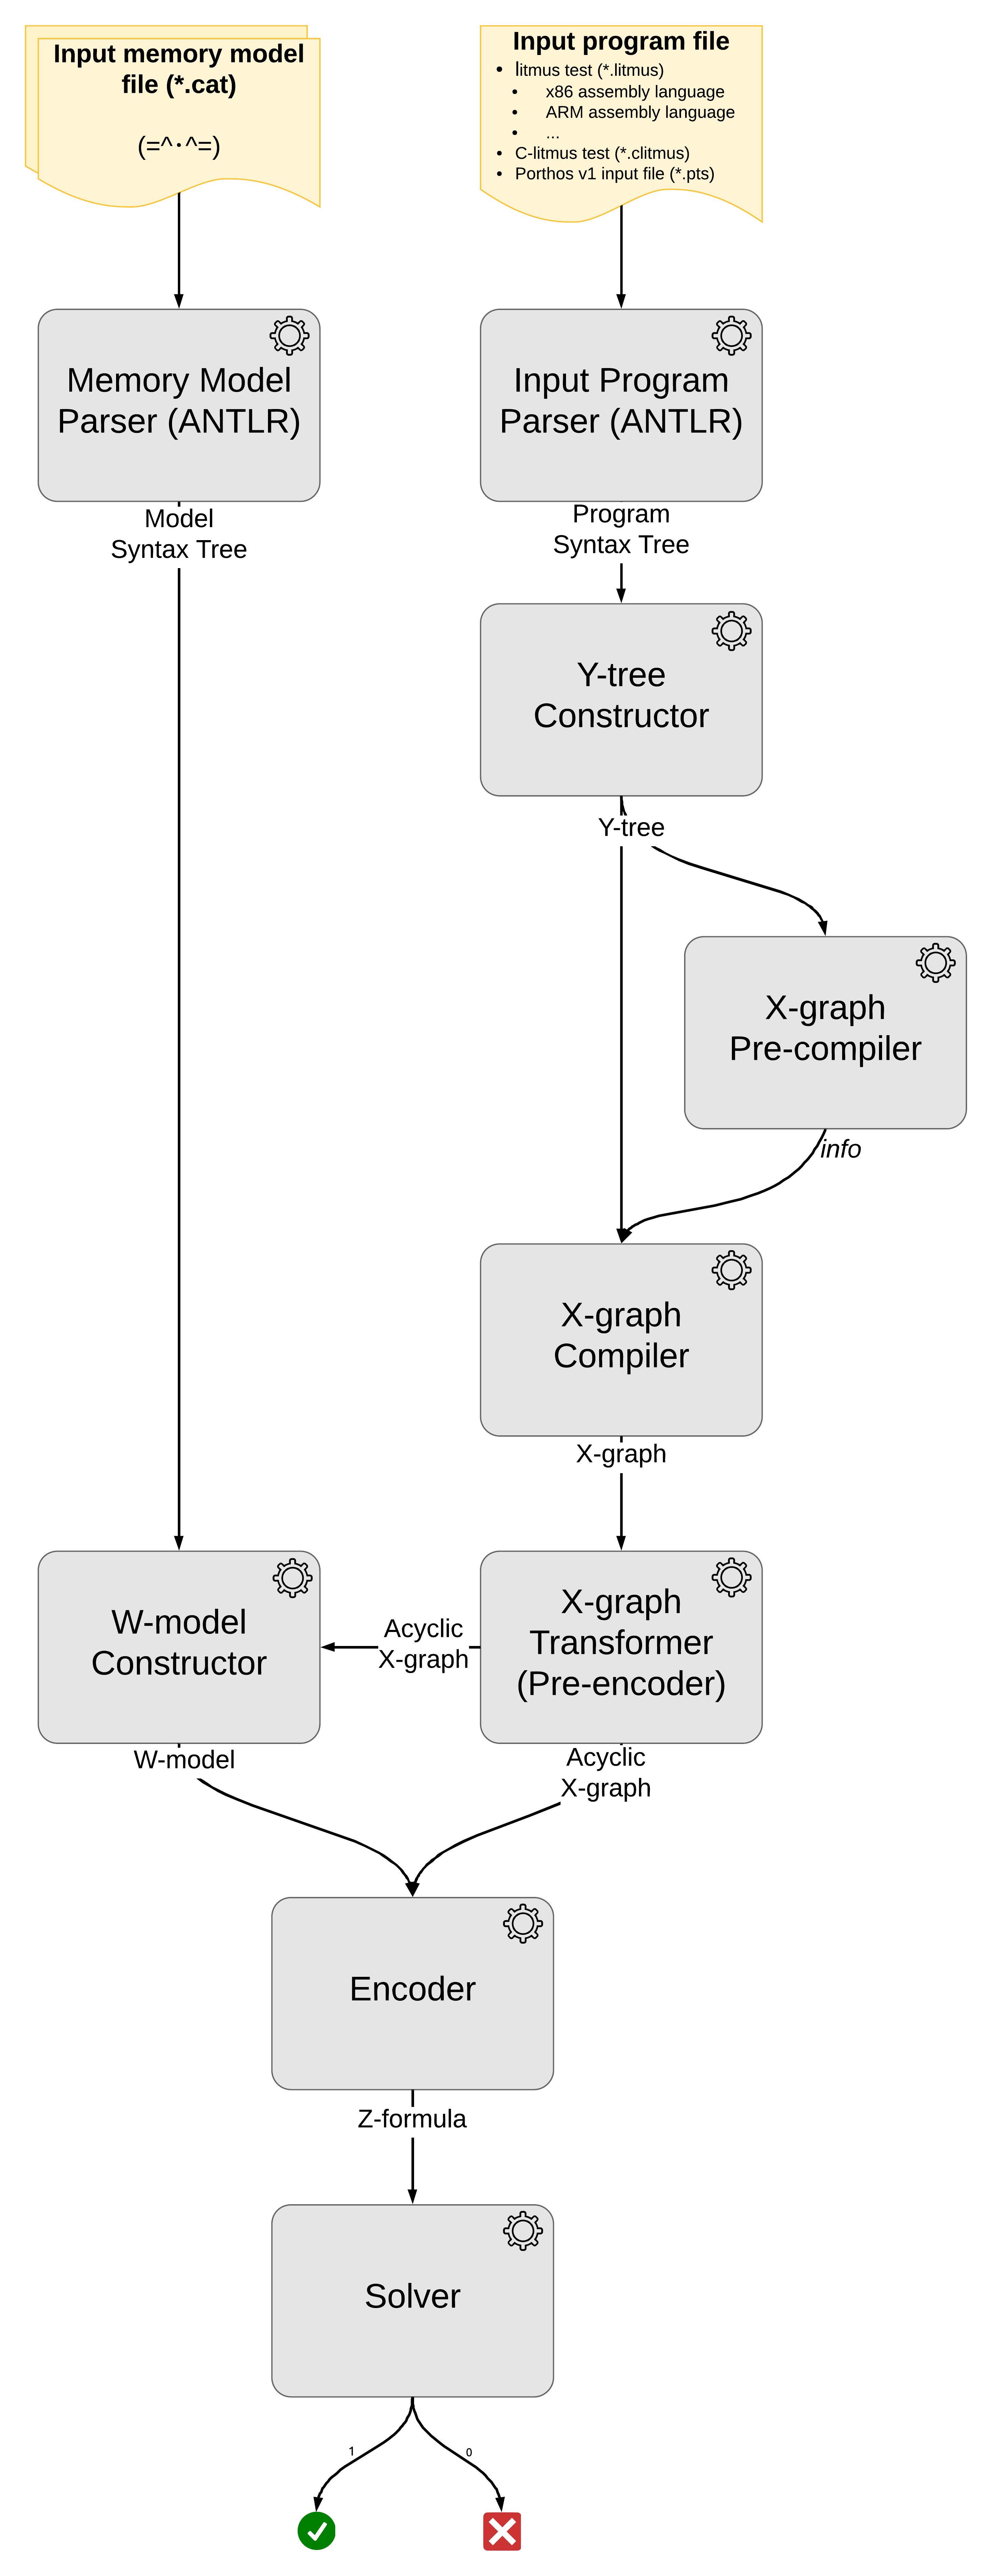
\includegraphics[width=\textwidth,height=\textheight,keepaspectratio]{img/my/lucidchart.com/data-flow-vert-300dpi.png}
  \caption{Main components of \porthos[2]}
  \label{fig:program-components}
\end{figure}


\section{The input language}
\label{ch:impl:input}

%TODO: say sth about 100500 litmus-tests for kernel

The previous version of \porthos processed the small subset of C as an input language (see grammar in Figure~\ref{syntax:in_grammar_pts})~\cite{Porthos17}.
It supported recursive definitions of control-flow instructions, that were directly encoded into SMT-formula.
The grammar supported by \porthos[2] was extended in order to support expressions valid in C. %TODO: examples, how imenno extended
Also, the input language of the first version of \porthos syntactically distinguished the type of a memory instruction (shared variable assignments were defined with symbol~`\texttt{:=}', and local variable assignments --- with symbol~`$\mathtt{\leftarrow}$'), whereas \porthos[2] determines the semantics of a function invocation during the preprocessing stage of compilation~(see Chapter~\ref{TODO!!!}).

\begin{figure}%[H]
%\begin{multicols}{2}
\begin{lstlisting}[mathescape=true,%
caption={Syntax of an input language of \porthos version 1},%
label={syntax:in_grammar_pts},%
literate={<--}{{$\leftarrow$}}1,%
morekeywords={if,then,else,return,while,program,thread,mfence,sync,lwsync,isync}%
breaklines=true,%
basicstyle=\ttfamily\scriptsize]
<prog> : program <thrd>*
       ;
<thrd> : thread <tid> <inst>
       ;
<inst> : <atom>
       | <inst> ; <inst>
       | while <pred> <inst>
       | if <pred > then <inst> else <inst>
       ;
<atom> : <reg> <-- <exp>
       | <reg> <-- <loc>
       | <loc> := <reg>
       | mfence
       | sync
       | lwsync
       | isync
       ;
\end{lstlisting}
%\end{multicols}
\end{figure}

Both \porthos and \porthos[2] \ use the parser generator ANTLR~\cite{parr2013definitive}, a powerful language processing tool.
The full ANTLR grammar of input language used by previous version of \porthos is available at Appendix~\ref{apx:in_grammar_pts}.
The \porthos[2] uses the C language grammar of proposed in the C11 standard~\cite{jtc2011sc22}, that was extended by litmus test-specific syntax such as initialisation and final-state assertion statements (the original ANTLR grammar can be found in the official ANTLR repository on GitHub~\footnote{The repository containing the collection of ANTLR v4 grammars:\\ \url{https://github.com/antlr/grammars-v4}}).
Current version of \porthos[2] can operate only in the inter-procedural mode, assuming that each function defined in the input file is being executed in a separate thread.
However, the redesigned architecture of \porthos[2] allow to easily support intra-procedural analysis by inlining function calls.


\subsection{Parsing the input}
\label{ch:impl:input-parser}

below: mostly mock text.

- The language-dependent syntax tree:
        - for now it's the C subset language which I called 'Cmin'; as a base, I used the C11 grammar from ANTLR github repository, then I simplified it a lot, cutting off many unnecessary C syntax features and making it more convenient for parsing. When developing the Cmin language, I kept in mind C elements that are necessary for processing the linux kernel code, though for now not the whole grammar element described in file 'Cmin.g4' are being implemented;
        - later I am going to add the litmus grammar as well;
        - in future, it will be not a problem to add any new C-like language;

- The language-independent abstract syntax tree (aliased 'Ytree', where 'Y' resembles branching of the tree):
        - all tree nodes in my code are prefixed with 'Y', see tentative (yet almost complete) class hierarchy in picture 'YEntity.png';
        - this AST contains very basic language elements according to the C execution model (statements and expressions);
        - converting the language-dependent syntax tree to the language-independent syntax tree is performed by Visitor pattern (e.g., for Cmin->Ytree conversion is made by 'CminToYtreeConverterVisitor')
        - minor changes are performed by converting to ytree representation: desugaring the target code, etc.


\section{Compiling the Y-tree to the X-graph}
\label{ch:impl:y2x}

\subsection{Preprocessing}
\label{ch:impl:y2x:preproc}
- Then, the AST is being interpreted and converted to event-based representation (aliased 'Xrepr' for eXecution representation):
        - more low-level code representation (or high-level assembly);
        - I try to keep this representation close to the one you described in your papers: basic load \& store events, branching events, fence events;
        - this representation is being implementing these days, I've just started doing it (see current class hierarchy in the picture 'XEntity.png');
        
- After we acquired the event-based representation, we can perform some modifications/simplifications/optimisations on it (separately, allowing user to manage them):
        - converting to SSA form as one of necessary steps before encoding;
        - (more? -- I'm not thinking about it yet);


\subsection{Compilation}
\label{ch:impl:y2x:compil}

\subsection{Loop unrolling}
\label{ch:impl:x2y:unrolling}
% If the analysing program contains a loop, then its control-flow graph represents the cyclic directed graph. Although, in order to be able to encode such a cyclic structure as a boolean formula, this graph needs to be  
% In order to be

The original program encoded into the \texttt{XGraph} represents a \textit{flow graph}, a connected cyclic directed graph with single source node \texttt{(ENTRY)} (usually for convenience all leaves are connected to the sink node \texttt{(EXIT)}). The cycles are caused by low-level jump instructions, obtained from non-linear high-level control-flow statements (such as \texttt{while}, \texttt{do-while}, \texttt{for}, etc.). However, the cyclic flow graph cannot be encoded into SMT formula since ...
//TODO:REFERENCE.%TODO



\begin{figure}
\begin{tikzpicture}[->,>=stealth',shorten >=1pt,auto,node distance=1.5cm,semithick]
\node[c] (1) [] {$1$};
\node[c] (2) [below left of=1] {$2$};
\node[c] (3) [below right of=1] {$3$};
\node[c] (4) [below of=3] {$4$};
\path[->]
(1) edge [] node {} (2)
(2) edge [bend left=50,dotted] node {} (1)
(1) edge [] node {} (3)
(3) edge [] node {} (4)
(4) edge [bend right=80,dotted] node {} (1)
;
\node[draw=none] (impl) [right=3cm of 3] {$\overset{k = 6}{\longmapsto}$};
;
\node[c] (21) [right=3cm of impl] {$2_1$};
\node[c] (11) [above right=1cm and 1cm of 21]{$1_1$};
\node[c] (31) [below right=1cm and 1cm of 11] {$3_1$};
\node[c] (41) [below of=31] {$4_1$};
\node[c] (12) [below of=21] {$1_2$};
\node[c] (22) [below left=1cm and 1cm of 12] {$2_2$};
\node[c] (32) [below right=1cm and 1cm of 12] {$3_2$};
\node[c] (13) [below of=41] {$1_3$};
\node[c] (14) [below of=22] {$1_4$};
\node[c] (43) [below of=32] {$4_3$};
\node[c] (23) [below of=13] {$2_3$};
\node[c] (33) [below of=13] {$3_3$};
\node[c] (24) [below left=1cm and 1cm of 14] {$2_4$};
\node[c] (34) [below right=1cm and 1cm of 14] {$3_4$};
\node[c] (15) [below right=1cm and -0.3cm of 43] {$1_5$};
\node[c] (44) [below of=33] {$4_4$};
\node[c] (6) [below left=1cm and 1cm of 15] {$6$};
\node[] (11k) [right=3.2cm of 11] {$(k = 1)$};
\node[] (31k) [right=1.7cm of 31] {$(k = 2)$};
\node[] (41k) [right=1.7cm of 41] {$(k = 3)$};
\node[] (13k) [right=1.7cm of 13] {$(k = 4)$};
\node[] (33k) [right=1.7cm of 33] {$(k = 5)$};
\node[] (44k) [right=1.7cm of 44] {$(k = 6)$};
\path[->]
(11) edge [] node {} (21)
(11) edge [] node {} (31)
(31) edge [] node {} (41)
(21) edge [] node {} (12)
(12) edge [bend right=10] node {} (22)
(12) edge [bend left=10] node {} (32)
(41) edge [] node {} (13)
(22) edge [] node {} (14)
(32) edge [] node {} (43)
(13) edge [] node {} (23)
(13) edge [] node {} (33)
(14) edge [bend right=10] node {} (24)
(14) edge [bend left=10] node {} (34)
(43) edge [] node {} (15)
(33) edge [bend right=10] node {} (15)
(33) edge [bend left=10] node {} (44)
(24) edge [bend right=20] node {} (6)
(34) edge [] node {} (6)
(15) edge [] node {} (6)
(44) edge [bend left=20] node {} (6)
;
\end{tikzpicture}
\label{fig:loop-unwind}
\caption{Example of the flow graph from Figure~\ref{fig:merged-loop.....}, unwinded up to the bound $k = 6$}
\end{figure}



\subsection{Input language parser}
\label{ch:impl:model-parser}


\section{XGraph to ZFormula (SMT) encoder}
\label{ch:impl:comp:zformula}

- Then, this modified event-representation is being encoded to SMT formula and sent to the solver.



% say something about equals() and hashCode()



\section{Optimisations}

... performed on each stage